\chapter{Statistics}

% \section{Introduction}

When running an experiment or conducting a survey we can potentially
end up with many hundreds, thousands or even millions of values in the
resulting data set. Too many data can be overwhelming and we need to
reduce them or represent them in a way that is easier to understand
and communicate.\par

Statistics is about summarising data. The methods of statistics allow
us to represent the essential information in a data set while
disregarding the unimportant information. We have to be careful to
make sure that we do not accidentally throw away some of the important
aspects of a data set.

%The figure below shows one example of how we can reduce the complexity
%of a data set while still retaining the important information.

%FIGURE: Side-by-side images of two data sets drawn from the same $2$-d
%normal distribution. $N = 50$. Even though the individual data are
%different, the statistics (central tendency and dispersion) are very
%similar. The statistics capture the interesting aspects of the data.
%\begin{center}
%  \begin{tikzpicture}
%  \end{tikzpicture}
%\end{center}
\par
By applying statistics properly we can highlight the important aspects
of data and make the data easier to interpret. By applying statistics
poorly or dishonestly we can also hide important information and let
people draw the wrong conclusions.\par

In this chapter we will look at a few numerical and graphical ways in
which data sets can be represented, to make them easier to interpret.
\chapterstartvideo{VMbqd}
\section{Collecting data}
\Definition{Data}{Data refer to the pieces of information that have
  been observed and recorded, from an experiment or a survey.}
\Note{The word {\em data} is the plural of the word {\em datum}, and
  therefore one should say, ``the data are'' and not ``the data is''.}

We distinguish between two main types of data: quantitative and
qualitative.

\Definition{Quantitative data}{Quantitative data are data that can be
  written as numbers.}

Quantitative data can be discrete or continuous. Discrete quantitative
data can be represented by integers and usually occur when we count
things, for example, the number of learners in a class, the number of
molecules in a chemical solution, or the number of SMS messages sent
in one day.\par

Continuous quantitative data can be represented by real numbers, for
example, the height or mass of a person, the distance travelled by a
car, or the duration of a phone call.

\Definition{Qualitative data}{Qualitative data are data that cannot be
  written as numbers.}

Two common types of qualitative data are categorical and anecdotal
data. Categorical data can come from one of a limited number of
possibilities, for example, your favourite cool drink, the colour of
your cell phone, or the language that you learned to speak at home.

Anecdotal data take the form of an interview or a story, for example,
when you ask someone what their personal experience was when using a
product, or what they think of someone else's behaviour.

Categorical qualitative data are sometimes turned into quantitative
data by counting the number of times that each category appears. For
example, in a class with $30$ learners, we ask everyone what the
colours of their cell phones are and get the following responses:

  \begin{center}
    \begin{tabular}{|c|c|c|c|c|c|c|c|c|c|}\hline
     
      black & black & black & white & purple & red & red & black & black & black \\ \hline
      white & white & black & black & black & black & purple & black & black & white \\ \hline
      purple & black & red & red & white & black & orange & orange & black & white \\ \hline
     
    \end{tabular}
  \end{center}

  This is a categorical qualitative data set since each of the
  responses comes from one of a small number of possible colours.

  We can represent exactly the same data in a different way, by
  counting how many times each colour appears.

  \begin{center}
    \begin{tabular}{|c|c|}\hline
      
      \textbf{Colour} & \textbf{Count} \\ \hline

      black & 15 \\
      white & 6 \\
      red & 4 \\
      purple & 3 \\
      orange & 2\\
    \hline
    \end{tabular}
  \end{center}

  This is a discrete quantitative data set since each count is an
  integer.

\begin{wex}{Qualitative and quantitative data}
{Thembisile is interested in becoming an airtime reseller to his
  classmates. He would like to know how much business he can expect
  from them. He asked each of his $20$ classmates how many SMS
  messages they sent during the previous day. The results were:
\\

    \begin{center}
      \begin{tabular}{|c|c|c|c|c|c|c|c|c|c|}\hline
        $20$ & $ 3$ & $ 0$ & $14$ & $30$ & $9$ & $11$ & $13$ & $13$ & $15$ \\ \hline
         $9$ & $13$ & $16$ & $12$ & $13$ & $7$ & $17$ & $14$ & $ 9$ & $13$ \\ \hline
        
      \end{tabular}
    \end{center}
    \vspace{8pt}\\

    Is this data set qualitative or quantitative? Explain your answer.
}{
\westep{Examine the data and answer the question}
  The number of SMS messages is a count represented by an integer, which means that it is
  quantitative and discrete.
}
\end{wex}

\begin{wex}{Qualitative and quantitative data}
{Thembisile would like to know who the most popular cellular
  provider is among learners in his school. This time Thembisile
  randomly selects $20$ learners from the entire school and asks them
  which cellular provider they currently use. The results were:

    \begin{center}
      \begin{tabular}{|p{0.17\textwidth}|p{0.17\textwidth}|p{0.17\textwidth}|p{0.17\textwidth}|p{0.17\textwidth}|}\hline
        
        Cell C & Vodacom & Vodacom & MTN & Vodacom \\\hline
        MTN & MTN & Virgin Mobile & Cell C & 8-ta \\\hline
        Vodacom & MTN & Vodacom & Vodacom & MTN \\\hline
        Vodacom & Vodacom & Vodacom & Virgin Mobile & MTN \\\hline
      \end{tabular}
    \end{center}
\vspace{8pt}\\
    Is this data set qualitative or quantitative? Explain your answer.
}{
\westep{Examine the data and answer the question}
  Since each response is not a number, but one of a small number of
  possibilities, these are categorical qualitative data.
}
\end{wex}

\section{Measures of central tendency}

\subsection{Mean}
\Definition{Mean}{The mean is the sum of a set of values,
  divided by the number of values in the set.  The notation for the
  mean of a set of values is a horizontal bar over the variable used
  to represent the set. The formula for the mean of a data set $\{x_1,
  x_2, \ldots, x_n\}$ is
  \begin{align*}
    \overline{x} &= \frac{1}{n}\sum_{i=1}^n x_i \\
                 &= \frac{x_1 + x_2 + \cdots + x_n}{n}
  \end{align*}
}
\mindsetvid{Mean, median and mode}{VMbqd}
The mean is sometimes also called the average or the arithmetic mean.

\begin{wex}{Calculating the mean}
{What is the mean of the data set $\{10;\ 20;\ 30;\ 40;\ 50\}$?}
{
  \westep{Calculate the sum of the data}
  \begin{equation*}
    10 + 20 + 30 + 40 + 50 = 150
  \end{equation*}

  \westep{Divide by the number of values in the data set to get the mean}

  Since there are $5$ values in the data set, the mean is
  \begin{equation*}
    \mbox{Mean} = \frac{150}{5} = 30
  \end{equation*}
}
\end{wex}

\subsection{Median}
\Definition{Median}
{The median of a data set is the value in the
  central position, when the data set has been arranged from the
  lowest to the highest value.}

Note that exactly half of the values from the data set are less than
  the median and the other half are greater than the median.\par

To calculate the median of a quantitative data set, first sort the
data from the smallest to the largest value and then find the value in
the middle. If there are an odd number of data, the median will be
equal to one of the values in the data set. If there are an even
number of data, the median will lie halfway between two values in
the data set.

\begin{wex}{Median for an odd number of values}
{What is the median of $\{10;\ 14;\ 86;\ 2;\ 68;\ 99;\ 1\}$?}
{
  \westep{Sort the values}

  The values in the data set, arranged from the smallest to the largest, are
  \begin{equation*}
    1;\ 2;\ 10;\ 14;\ 68;\ 86;\ 99
  \end{equation*}

  \westep{Find the number in the middle}

  There are $7$ values in the data set. Since there are an odd number
  of values, the median will be equal to the value in the middle,
  namely, in the $4^{\mathrm{th}}$ position. The value in the $4^{\mathrm{th}}$ position is
  $14$ and therefore the median of the data set is $14$.
}
\end{wex}

\begin{wex}{Median for an even number of values}
{What is the median of $\{11;\ 10;\ 14;\ 86;\ 2;\ 68;\ 99;\ 1\}$?}
{
  \westep{Sort the values}

  The values in the data set, arranged from the smallest to the largest, are
  \begin{equation*}
    1;\ 2;\ 10;\ 11;\ 14;\ 68;\ 86;\ 99
  \end{equation*}

  \westep{Find the number in the middle}

  There are $8$ values in the data set. Since there are an even number
  of values, the median will be halfway between the two values in the
  middle, namely, between the $4^{\mathrm{th}}$ and $5^{\mathrm{th}}$ positions. The value in the
  $4^{\mathrm{th}}$ position is $11$ and the value in the $5^{\mathrm{th}}$ position is
  $14$. The median lies halfway between these two values and is
  therefore
  \begin{equation*}
    \mbox{Median} = \frac{11+14}{2} = 12,5
  \end{equation*}
}
\end{wex}

\subsection{Mode}
\Definition{Mode}
{The mode of a data set is the value that occurs most often in the
  set. The mode can also be described as the most frequent or most
  common value in the data set.}

To calculate the mode, we simply count the number of times that each
value appears in the data set and then find the value that appears
most often.

A data set can have more than one mode if there is more than one value
with the highest count. For example, both $2$ and $3$ are modes in the
data set $\{1;\ 2;\ 2;\ 3;\ 3\}$. If all points in a data set occur
with equal frequency, it is equally accurate to describe the data set
as having many modes or no mode.

\begin{wex}{Finding the mode}
{Find the mode of the data set $\{2;\ 2;\ 3;\ 4;\ 4;\ 4;\ 6;\ 6;\ 7;\ 8;\ 8;\ 10;\ 10\}$.}
{
  \westep{Count the number of times that each value appears in the data
    set}
\\
  \begin{center}
    \begin{tabular}{|c|c|} \hline
      \textbf{Value} & \textbf{Count} \\ \hline

      $2$ & $2$ \\ \hline
      $3$ & $1$ \\\hline 
      $4$ & $3$ \\\hline
      $6$ & $2$ \\\hline
      $7$ & $1$ \\\hline
      $8$ & $2$ \\\hline
      $10$ & $2$ \\\hline

    \end{tabular}
  \end{center}

  \westep{Find the value that appears most often}

  From the table above we can see that $4$ is the only value that
  appears $3$ times, and all the other values appear less
  often. Therefore the mode of the data set is $4$.
}
\end{wex}

One problem with using the mode as a measure of central tendency is
that we can usually not compute the mode of a continuous data
set. Since continuous values can lie anywhere on the real line, any
particular value will almost never repeat. This means that the
frequency of each value in the data set will be $1$ and that there will
be no mode. We will look at one way of addressing this problem in
the section
% \ref{sec:statistics_grouping_data} 
on grouping data.

\begin{wex}{Comparison of measures of central tendency}
{There are regulations in South Africa related to bread production
    to protect consumers. By law, if a loaf of bread is not labelled,
    it must weigh $800$ g, with the leeway of $5$ percent under or $10$
    percent over.  Vishnu is interested in how a well-known, national
    retailer measures up to this standard. He visited his local branch
    of the supplier and recorded the masses of $10$ different loaves
    of bread for one week. The results, in grams, are given below:\\

    \begin{center}
      \begin{tabular}{|c|c|c|c|c|c|c|} \hline
       
        \textbf{Monday} & \textbf{Tuesday} & \textbf{Wednesday} & \textbf{Thursday} & \textbf{Friday} & \textbf{Saturday} & \textbf{Sunday} \\ \hline
        
        $802,4$ & $787,8$ & $815,7$ & $807,4$ & $801,5$ & $786,6$ & $799,0$ \\ \hline
        $796,8$ & $798,9$ & $809,7$ & $798,7$ & $818,3$ & $789,1$ & $806,0$ \\ \hline
        $802,5$ & $793,6$ & $785,4$ & $809,3$ & $787,7$ & $801,5$ & $799,4$ \\ \hline
        $819,6$ & $812,6$ & $809,1$ & $791,1$ & $805,3$ & $817,8$ & $801,0$ \\ \hline
        $801,2$ & $795,9$ & $795,2$ & $820,4$ & $806,6$ & $819,5$ & $796,7$ \\ \hline
        $789,0$ & $796,3$ & $787,9$ & $799,8$ & $789,5$ & $802,1$ & $802,2$ \\ \hline
        $789,0$ & $797,7$ & $776,7$ & $790,7$ & $803,2$ & $801,2$ & $807,3$ \\ \hline
        $808,8$ & $780,4$ & $812,6$ & $801,8$ & $784,7$ & $792,2$ & $809,8$ \\ \hline
        $802,4$ & $790,8$ & $792,4$ & $789,2$ & $815,6$ & $799,4$ & $791,2$ \\ \hline
        $796,2$ & $817,6$ & $799,1$ & $826,0$ & $807,9$ & $806,7$ & $780,2$ \\ \hline
       
      \end{tabular}
    \end{center}
\vspace{8pt}\\
    \begin{enumerate}[noitemsep, label=\textbf{\arabic*}.]
    \item Is this data set qualitative or quantitative? Explain your
      answer.
    \item Determine the mean, median and mode of the mass of a loaf of bread
      for each day of the week. Give your answer correct to $1$ decimal place.
    \item Based on the data, do you think that this supplier is
      providing bread within the South African regulations?
    \end{enumerate}
}{
  \westep{Qualitative or quantitative?}

  Since each mass can be represented by a number, the data
  set is quantitative. Furthermore, since a mass can be any real
  number, the data are continuous.

  \westep{Calculate the mean}

  In each column (for each day of the week), we add up the
  measurements and divide by the number of measurements, $10$.

  For Monday, the sum of the measured values is $8007,9$ and so the
  mean for Monday is
  \begin{equation*}
    \frac{8007,9}{10} = 800,8\mbox{ g}
  \end{equation*}

  In the same way, we can compute the mean for each day of the
  week. See the table below for the results.

  \westep{Calculate the median}

  In each column we sort the numbers from lowest to highest and find
  the value in the middle. Since there are an even number of
  measurements ($10$), the median is halfway between the two numbers in
  the middle.

  For Monday, the sorted list of numbers is
  \begin{equation*}
    789,0;\ 789,0;\ 796,2;\ 796,7;\ 801,2;\ 802,3;\ 802,3;\ 802,5;\ 808,7;\ 819,6
  \end{equation*}
  The two numbers in the middle are $801,2$ and $802,3$ and so the
  median is
  \begin{equation*}
    \frac{801,2 + 802,3}{2} = 801,8\mbox{ g}
  \end{equation*}

  In the same way, we can compute the median for each day of the
  week:
\\
  \begin{center}
    \begin{tabular}{|c|c|c|} \hline
      \textbf{Day} & \textbf{Mean} &\textbf{Median} \\  \hline
      Monday & $800,8$ g & $801,8$ g \\ \hline
      Tuesday & $797,2$ g & $796,1$ g \\ \hline
      Wednesday & $798,4$ g & $797,2$ g \\ \hline
      Thursday & $803,4$ g & $800,8$ g \\ \hline
      Friday & $802,0$ g & $804,3$ g \\ \hline
      Saturday & $801,6$ g & $801,4$ g \\ \hline
      Sunday & $799,3$ g & $800,2$ g \\ \hline
    \end{tabular}
  \end{center}
\vspace{8pt}\\
  From the above calculations we can see that the means and medians
  are close to one another, but not quite equal. In the next worked
  example we will see that the mean and median are not always
  close to each other.

  \westep{Determine the mode}

  Since the data are continuous we cannot compute the mode. In the next
  section we will see how we can group data in order to make it possible
  to compute an approximation for the mode.

  \westep{Conclusion: Is the supplier reliable?}

  From the question, the requirements are that the mass of a loaf of
  bread be between $800$ g minus $5$\%, which is $760$ g, and plus
  $10$\%, which is $880$ g. Since every one of the measurements made
  by Vishnu lies within this range and since the means and medians are
  all close to $800$ g, we can conclude that the supplier is reliable.
}
\end{wex}

\Definition{Outlier}{An outlier is a value in the data set that is not
  typical of the rest of the set. It is usually a value that is much
  greater or much less than all the other values in the data set.}

\begin{wex}{Effect of outliers on mean and median}
{The heights of $10$ learners are measured in centimetres to obtain
    the following data set:
    \begin{equation*}
      \{150;\ 172;\ 153;\ 156;\ 146;\ 157;\ 157;\ 143;\ 168;\ 157\}
    \end{equation*}
    Afterwards, we include one more learner in the group, who is
    exceptionally tall at $181$ cm.

    Compare the mean and median of the heights of the learners before
    and after the $11^{\mathrm{th}}$ learner was included.
}{
  \westep{Calculate the mean of the first $10$ learners}

  \begin{align*}
    \mbox{Mean } &=\frac{150 + 172 + 153 + 156 + 146 + 157 + 157 + 143 + 168 + 157}{10}\\
    &= 155,9\mbox{ cm}
  \end{align*}

  \westep{Calculate the mean of all $11$ learners}

  \begin{equation*}
    \mbox{Mean } &= \frac{150 + 172 + 153 + 156 + 146 + 157 + 157 + 143 + 168 + 157 + 181}{11}\\
    &= 158,2\mbox{ cm}
  \end{equation*}

  From this we see that the average height changes by
  $158,2 - 155,9 = 2,3\mbox{ cm}$ when we introduce
  the outlier value (the tall person) to the data set.

  \westep{Calculate the median of the first $10$ learners}

  To find the median, we need to sort the data set:
  \begin{equation*}
    \{143;\ 146;\ 150;\ 153;\ 156;\ 157;\ 157;\ 157;\ 168;\ 172\}
  \end{equation*}
  Since there are an even number of values, $10$, the median
  lies halfway between the $5^{\mathrm{th}}$ and $6^{\mathrm{th}}$ values:
  \begin{equation*}
    \mbox{Median} =\frac{156+157}{2} = 156,5\mbox{ cm}
  \end{equation*}

  \westep{Calculate the median of all $11$ learners}

  After adding the tall learner, the sorted data set is
  \begin{equation*}
    \{143;\ 146;\ 150;\ 153;\ 156;\ 157;\ 157;\ 157;\ 168;\ 172;\ 181\}
  \end{equation*}
  Now, with $11$ values, the median is the $6^{\mathrm{th}}$ value: $157$ cm.
  So, the median changes by only $0,5$ cm when we add the outlier
  value to the data set.

  In general, the median is less affected by the addition of outliers
  to a data set than the mean is. This is important because it is
  quite common that outliers are measured during an experiment,
  because of problems with the equipment or unexpected interference.
}
\end{wex}

\begin{exercises}{}{
    \begin{enumerate}[noitemsep, label=\textbf{\arabic*}.]
    \item Calculate the mean, median and mode of the following data sets:
      \begin{enumerate}[noitemsep, label=\textbf{(\alph*)} ]
      \item $2;~5;~8;~8;~11;~13;~22;~23;~27$
      \item $15;~17;~24;~24;~26;~28;~31;~43$
      \item $4;~11;~3;~15;~11;~13;~25;~17;~2;~11$
      \item $24;~35;~28;~41;~32;~49;~31$
      \end{enumerate}
    \item The ages of $15$ runners of the Comrades Marathon were recorded:
      \begin{equation*}
        31;~42;~28;~38;~45;~51;~33;~29;~42;~26;~34;~56;~33;~46;~41
      \end{equation*}
      Calculate the mean, median and modal age.
    \item In the first of a series of jars, there is $1$ sweet. In the
      second jar, there are $3$ sweets. The mean number of sweets in the
      first two jars is $2$.
      \begin{enumerate}[noitemsep, label=\textbf{(\alph*)} ]
      \item If the mean number of sweets in the first three jars is $3$, how
        many sweets are there in the third jar?
      \item If the mean number of sweets in the first four jars is $4$, how
        many sweets are there in the fourth jar?
      \end{enumerate}
    \item Find a set of five ages for which the mean age is $5$, the modal
      age is $2$ and the median age is $3$ years.
    \item Four friends each have some marbles. They work out that the mean
      number of marbles they have is $10$. One friend leaves with $4$
      marbles. How many marbles do the remaining friends have together?
    \end{enumerate}
\practiceinfo
\par 
\par \begin{tabular}[h]{cccccc}
(1.) 00jr&  (2.) 00js&  (3.) 00jt&  (4.) 00ju&  (5.) 00jv\end{tabular}
}
\end{exercises}

\section{Grouping data}
\label{sec:statistics_grouping_data}
A common way of handling continuous quantitative data is to subdivide
the full range of values into a few sub-ranges.
By assigning each continuous value to the sub-range within which it
falls, the data set changes from continuous to discrete.\par
%We will see below that this has some benefits, but we gain the
%benefits at the cost of losing some information.
\mindsetvid{Grouping data}{VMbue}
Grouping is done by defining a set of ranges and then counting how
many of the data fall inside each range. The sub-ranges must
 not overlap and must cover the entire
range of the data set.\par

One way of visualising grouped data is as a histogram. A histogram is
a collection of rectangles, where the base of a rectangle (on the
$x$-axis) covers the values in the range associated with it, and the
height of a rectangle corresponds to the number of values in its
range.

\begin{wex}{Groups and histograms}
{The heights in centimetres of $30$ learners are given below.
\\
    \begin{center}
      \begin{tabular}{|c|c|c|c|c|c|c|c|c|c|}\hline
   
        142 & 163 & 169 & 132 & 139 & 140 & 152 & 168 & 139 & 150\\ \hline
        161 & 132 & 162 & 172 & 146 & 152 & 150 & 132 & 157 & 133\\ \hline
        141 & 170 & 156 & 155 & 169 & 138 & 142 & 160 & 164 & 168\\\hline
 
      \end{tabular}
    \end{center}
\vspace {8pt}\\
    Group the data into the following ranges and draw a histogram of the
    grouped data:
    \begin{align*}
      130 &\leq h < 140 \\
      140 &\leq h < 150 \\
      150 &\leq h < 160 \\
      160 &\leq h < 170 \\
      170 &\leq h < 180
    \end{align*}
    (Note that the ranges do not overlap since each one starts where
    the previous one ended.)
}{
  \westep{Count the number of values in each range}
  \begin{center}
    \begin{tabular}{|c|c|} \hline

      \textbf{Range} & \textbf{Count} \\ \hline
    
      $130 \leq h < 140$ & $7$ \\ \hline
      $140 \leq h < 150$ & $5$ \\\hline
      $150 \leq h < 160$ & $7$ \\\hline
      $160 \leq h < 170$ & $9$ \\\hline
      $170 \leq h < 180$ & $2$ \\\hline

    \end{tabular}
  \end{center}
  
  \westep{Draw the histogram}

  Since there are $5$ ranges, the histogram will have $5$
  rectangles. The base of each rectangle is defined by its range. The
  height of each rectangle is determined by the count in its range.
  
  \begin{center}
    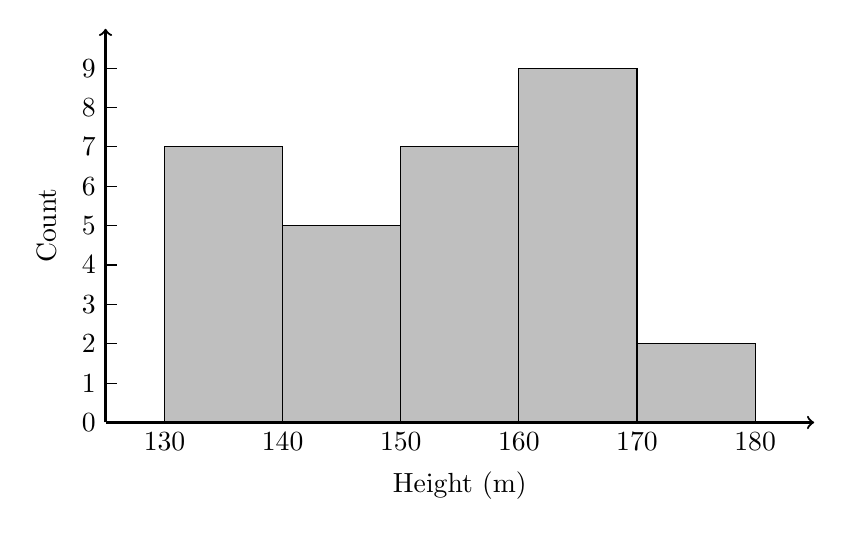
\begin{tikzpicture}[xscale=0.15,yscale=0.5]
      \draw[fill=lightgray] (130,0) rectangle (140,7);
      \draw[fill=lightgray] (140,0) rectangle (150,5);
      \draw[fill=lightgray] (150,0) rectangle (160,7);
      \draw[fill=lightgray] (160,0) rectangle (170,9);
      \draw[fill=lightgray] (170,0) rectangle (180,2);

\draw[thick,->] (125,0) -- (185,0) node[anchor=north] {};
      % x labels
      \foreach \x in {130, 140, ..., 180} {
        \draw (\x,0) node[anchor=north] {$\x$};
      }

      % y axis
      \draw[thick,->] (125,0) -- (125,10) node[midway,sloped,anchor=south,yshift=0.5cm] {Count};
      % y labels
      \foreach \y in {0, 1, ..., 9} {
        \draw (125,\y) node[anchor=east] {$\y$} -- (126,\y);
      }
      % axis labels
      \draw (155, -1) node[anchor=north] {Height (m)};
    \end{tikzpicture}
  \end{center}

  The histogram makes it easy to see in which range most of the
  heights are located and provides an overview of the distribution of
  the values in the data set.
}
\end{wex}    

\begin{exercises}{}{
    \begin{enumerate}[itemsep=5pt, label=\textbf{\arabic*}. ]
    \item  A class experiment was conducted and $50$ learners were asked to
      guess the number of sweets in a jar. The following guesses were
      recorded:
      \\
      \begin{center}
        \begin{tabular}{|c|c|c|c|c|c|c|c|c|c|} \hline
          56 & 49 & 40 & 11 & 33 & 33 & 37 & 29 & 30 & 59 \\ \hline
          21 & 16 & 38 & 44 & 38 & 52 & 22 & 24 & 30 & 34 \\\hline
          42 & 15 & 48 & 33 & 51 & 44 & 33 & 17 & 19 & 44 \\\hline
          47 & 23 & 27 & 47 & 13 & 25 & 53 & 57 & 28 & 23 \\\hline
          36 & 35 & 40 & 23 & 45 & 39 & 32 & 58 & 22 & 40 \\\hline
        \end{tabular}
      \end{center}
      \vspace{8pt}\\

      \begin{enumerate}[noitemsep, label=\textbf{(\alph*)} ]
      \item
        Draw up a grouped frequency table using the intervals
        $10 < x \leq 20$;\ $20 < x \leq 30$;\ $30 < x \leq 40$;\ 
        $40 < x \leq 50$;and \ $50 < x \leq 60$.
      \item Draw the histogram corresponding to the frequency table of the
        grouped data.
      \end{enumerate}
    \end{enumerate}
\practiceinfo
\par 
\par \begin{tabular}[h]{cccccc}
(1.) 00jw& \end{tabular}
}
\end{exercises}
% 
 %Put this in other text flows straight out of previous exercises?!?!
\subsection*{Measures of central tendency}
With grouped data our estimates of central tendency will change
because we lose some information when we place each value in a range.
If all we have to work with is the grouped data, we do not know the
measured values to the same accuracy as before. The best we can do is
to assume that values are grouped at the centre of each range.\par

Looking back to the previous worked example, we started with this data
set of learners' heights.
\begin{align*}
  \{&132;\ 132;\ 132;\ 133;\ 138;\ 139;\ 139;\ 140;\ 141;\ 142;\ 142;\ 146;\ 150;\ 150;\ 152;\\
    &152;\ 155;\ 156;\ 157;\ 160;\ 161;\ 162;\ 163;\ 164;\ 168;\ 168;\ 169;\ 169;\ 170;\ 172\}
\end{align*}
Note that the data are sorted.

The mean of these data is $151,8$ and the median is $152$. The mode is
$132$, but remember that there are problems with computing the mode of
continuous quantitative data.\par

After grouping the data, we now have the data set shown below. Note
that each value is placed at the centre of its range and that the
number of times that each value is repeated corresponds exactly to the
counts in each range.
\begin{align*}
  \{&135;\ 135;\ 135;\ 135;\ 135;\ 135;\ 135;\ 145;\ 145;\ 145;\ 145;\ 145;\ 155;\ 155;\ 155;\\
    &155;\ 155;\ 155;\ 155;\ 165;\ 165;\ 165;\ 165;\ 165;\ 165;\ 165;\ 165;\ 165;\ 175;\ 175\}
\end{align*}
The grouping changes the measures of central tendency since each datum
is treated as if it occurred at the centre of the range in which it was
placed.\par

The mean is now $153$, the median $155$ and the mode is $165$. This is
actually a better estimate of the mode, since the grouping showed in
which range the learners' heights were clustered.


\begin{exercises}{}{
  \begin{enumerate}[itemsep=8pt, label=\textbf{\arabic*}.]

  \item Consider the following grouped data and calculate the mean,
    the modal group and the median group.
\\
    \begin{center}
      \begin{tabular}{|c|c|}\hline
      
        \textbf{Mass (kg)} & \textbf{Count} \\\hline
     
        $40 < m \leq 45$ & $7$ \\\hline
        $45 < m \leq 50$ & $10$ \\\hline
        $50 < m \leq 55$ & $15$ \\\hline
        $55 < m \leq 60$ & $12$ \\\hline
        $60 < m \leq 65$ & $6$ \\\hline
  
      \end{tabular}
    \end{center}

  \item Find the mean, the modal group and the median group in this
    data set of how much time people needed to complete a game.
\\
    \begin{center}
      \begin{tabular}{|c|c|} \hline

       \textbf{Time (s)} & \textbf{Count} \\ \hline

        $35 < t \leq 45$ & $5$ \\\hline
        $45 < t \leq 55$ & $11$ \\\hline
        $55 < t \leq 65$ & $15$ \\\hline
        $65 < t \leq 75$ & $26$ \\\hline
        $75 < t \leq 85$ & $19$ \\\hline
        $85 < t \leq 95$ & $13$ \\\hline
        $95 < t \leq 105$ & $6$ \\\hline

      \end{tabular}
    \end{center}
\item The histogram below shows the number of passengers that travel in Alfred's minibus taxi per week.\\
Calculate
\begin{enumerate}[noitemsep, label=\textbf{(\alph*)} ]
\item the modal interval
\item the total number of passengers to travel in Alfred's taxi
\item an estimate of the mean
\item an estimate of the median
\item if it is estimated that every passenger travelled an average distance of $5$ km, how much money would Alfred have made if he charged R~$3,50$ per km?
\end{enumerate}
\begin{center}
\scalebox{1} % Change this value to rescale the drawing.
{
\begin{pspicture}(0,-5.1475)(9.378126,5.1075)
\definecolor{color5165b}{rgb}{0.7725490196078432,0.7725490196078432,0.7725490196078432}
\rput(1.3781264,-3.8925){\psaxes[linewidth=0.028222222,arrowsize=0.05291667cm 2.0,arrowlength=1.4,arrowinset=0.4,tickstyle=bottom,ticksize=0.10583333cm,dx=1.0cm,dy=1.0cm,Dx=100,Dy=2,Ox=300]{<->}(0,0)(-1,-1)(8,9)}
\psframe[linewidth=0.02,dimen=outer,fillstyle=solid,fillcolor=color5165b](3.392293,-1.8890625)(2.372293,-3.8890624)
\psframe[linewidth=0.02,dimen=outer,fillstyle=solid,fillcolor=color5165b](4.412293,-0.8890625)(3.372293,-3.8890624)
\psframe[linewidth=0.02,dimen=outer,fillstyle=solid,fillcolor=color5165b](5.412293,2.1309376)(4.372293,-3.8890624)
\psframe[linewidth=0.02,dimen=outer,fillstyle=solid,fillcolor=color5165b](6.392293,4.1309376)(5.372293,-3.8890624)
\psframe[linewidth=0.02,dimen=outer,fillstyle=solid,fillcolor=color5165b](7.392293,0.1309375)(6.372293,-3.8890624)
\psframe[linewidth=0.02,dimen=outer,fillstyle=solid,fillcolor=color5165b](8.392293,-2.8690624)(7.372293,-3.8890624)
% \usefont{T1}{ptm}{m}{n}
\rput(5.369637,-4.9225){No.\@{} of passengers}
% \usefont{T1}{ptm}{m}{n}
\rput{89.854546}(0.73185694,0.38878262){\rput(0.13573053,0.5775){Count}}
\end{pspicture} 
}
\end{center}
  \end{enumerate}

\practiceinfo
\par 
\par \begin{tabular}[h]{cccccc}
(1.) 00jx&  (2.) 00jy&  (3.) 00jz\end{tabular}

}
\end{exercises}

\section{Dispersion}
The central tendency is not the only interesting or useful information
about a data set. The two data sets illustrated below have the same mean ($0$),
but have different spreads
    around the mean. Each circle represents one datum.
\mindsetvid{Range and other measures of dispersion}{VMbsf}
\begin{figure}[H]
  \begin{center}
    \begin{tabular}{cc}
      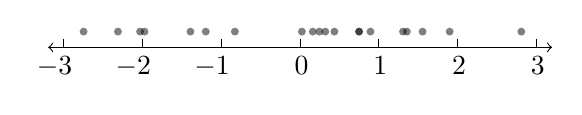
\begin{tikzpicture}
        \draw[<->] (-3.2, -0.2) -- (3.2, -0.2);
        \foreach \x in {-3, ..., 3} {
          \draw (\x, -0.2) -- (\x, -0.1);
          \draw (\x, -0.2) node[anchor=north east,xshift=0.23cm] {$\x$};
        }
        \foreach \x in {1.555, 1.899, 0.893, 0.160, 0.244, -0.829,
                        -1.199, -2.750, 0.022, -2.314, 2.809, 0.319,
                        -2.033, -1.976, 1.355, 0.749, 0.435, -1.393,
                        0.748, 1.306} {
          \fill[black,fill opacity=0.5] (\x,0) circle (0.05cm);
        }
      \end{tikzpicture}
      &
      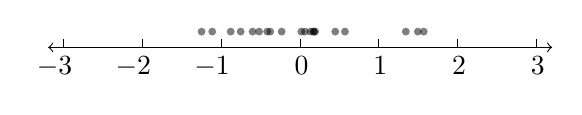
\begin{tikzpicture}
        \draw[<->] (-3.2, -0.2) -- (3.2, -0.2);
        \foreach \x in {-3, ..., 3} {
          \draw (\x, -0.2) -- (\x, -0.1);
          \draw (\x, -0.2) node[anchor=north east,xshift=0.23cm] {$\x$};
        }
        \foreach \x in {0.015, -0.418, 1.494, -0.882, 0.446, 0.061,
                        1.570, -0.755, 0.174, -0.604, -1.116, -0.380,
                        0.133, 0.569, -0.235, -0.521, 0.191, 0.169,
                        -1.252, 1.342} {
          \fill[black,fill opacity=0.5] (\x,0) circle (0.05cm);
        }
      \end{tikzpicture}
    \end{tabular}
  \end{center}
%   \begin{caption*}\end{caption*}
\end{figure}

 Dispersion is
a general term for different statistics that describe how values are
distributed around the centre. In this section we will look at measures of dispersion.

\subsection{Range}
\Definition{Range}{The range of a data set is the difference between
  the maximum and minimum values in the set.}

The most straightforward measure of dispersion is the range. The range
simply tells us how far apart the largest and smallest values in a
data set are. The range is very sensitive to outliers.

\begin{wex}{Range}
{Find the range of the following data set:
    \begin{equation*}
      \{1;\ 4;\ 5;\ 8;\ 6;\ 7;\ 5;\ 6;\ 7;\ 4;\ 10;\ 9;\ 10\}
    \end{equation*}
    What would happen if we removed the first datum from the set?
}{
  \westep{Find the minimum value}
  The smallest value in the data set is $1$.

  \westep{Find the maximum value}
  The largest value in the data set is $10$.

  \westep{Subtract the minimum value from the maximum value}
  The range is $10-1=9$.

  \westep{Remove the first datum}
  If the first datum, $1$, were to be removed from the set, the
  minimum value would be $4$. This means that the range would change
  to $10-4=6$. This is very different from the previous value. This
  shows that the range is sensitive to outliers. In the data set
  above, the value $1$ is not typical of the other values. It is an
  outlier and has a big influence on the range.
}
\end{wex}


\subsection{Percentiles}

\Definition{Percentile}{The $p^{\mathrm{th}}$ percentile is the value, $v$, that
  divides a data set into two parts, such that $p$ per cent of the
  values in the data set are less than $v$ and $100-p$ per cent of the
  values are greater than $v$. Percentiles can lie in the range $0 \leq
  p \leq 100$.}

To understand percentiles properly, we need to distinguish between $3$
different aspects of a datum: its value, its rank and its
percentile:
\begin{itemize}
 \item The value of a datum is what we measured and recorded
during an experiment or survey. 
\item The rank of a datum is its position in
the sorted data set (for example, first, second, third, and so
on). 
\item The percentile at which a particular datum is, tells us what
percentage of the values in the full data set are less than this
datum.
\end{itemize}
\par
  The table below summarises the value, rank and percentile of the
  data set
  \begin{equation*}
    \{14,2;\ 13,9;\ 19,8;\ 10,3;\ 13,0;\ 11,1\}
  \end{equation*}

  \begin{center}
    \begin{tabular}{|c|c|c|} \hline

      \textbf{Value} & \textbf{Rank} & \textbf{Percentile} \\\hline

      $10,3$  & $1$    & $0$ \\\hline
      $11,1$  & $2$    & $20$ \\\hline
      $13,0$  & $3$    & $40$ \\\hline
      $13,9$  & $4$    & $60$ \\\hline
      $14,2$  & $5$    & $80$ \\\hline
      $19,8$  & $6$    & $100$ \\\hline

    \end{tabular}
  \end{center}

 As an example, $13,0$ is at the $40^{\mathrm{th}}$ percentile since there are
  $2$ values less than $13,0$ and $3$ values greater than $13,0$.
  \begin{equation*}
    \frac{2}{2+3} = 0,4 = 40\%
  \end{equation*}
% \end{example}

In general, the formula for finding the $p^{\mathrm{th}}$ percentile in an ordered
data set with $n$ values is
\begin{equation*}
  r = \frac{p}{100}\left(n-1\right)+1
\end{equation*}
This gives us the rank, $r$, of the $p^{\mathrm{th}}$ percentile. To find the
value of the $p^{\mathrm{th}}$ percentile, we have to count from the first value in
the ordered data set up to the $r^{\mathrm{th}}$ value.

Sometimes the rank will not be an integer. This means that the
percentile lies between two values in the data set. The convention is
to take the value halfway between the two values indicated by the
rank.

The figure below shows the relationship between rank and percentile
graphically. We have already encountered three percentiles in this
chapter: the median, the minimum and the maximum.

\begin{center}
  \begin{tikzpicture}[xscale=0.1]
    \draw (0,0) -- (100,0);
    \foreach \p in {0, 25, ..., 100} {
      \draw (\p, -0.1) -- (\p, 0.1);
    }
    \draw (0, -0.1) node[anchor=north east,xshift=-0.35cm,yshift=-0.05cm] {$p$};
    \draw (0, -0.1) node[anchor=north] {$0$};
    \draw (50, -0.1) node[anchor=north] {$50$};
    \draw (100, -0.1) node[anchor=north] {$100$};
    \draw (0, -0.75) node[anchor=north] {minimum};
    \draw (50, -0.75) node[anchor=north] {median};
    \draw (100, -0.75) node[anchor=north] {maximum};
    \draw (0, +0.1) node[anchor=south east,xshift=-0.35cm,yshift=+0.05cm] {$r$};
    \draw (0, +0.1) node[anchor=south] {$1$};
    \draw (50, +0.1) node[anchor=south] {$\dfrac{n+1}{2}$};
    \draw (100, +0.1) node[anchor=south] {$n$};
  \end{tikzpicture}
\end{center}

The median is defined as the value halfway in a sorted data set. Since
$50\% = \frac{1}{2}$, the median is exactly the same as the $50^{\mathrm{th}}$
percentile.  The minimum value is by definition the smallest and
therefore the leftmost value in a sorted set. This makes the minimum
equivalent to the $0^{\mathrm{th}}$ percentile. Similarly, the maximum is
equivalent to the $100^{\mathrm{th}}$ percentile.

\begin{wex}{Using the percentile formula}
{Determine the minimum, maximum and median values of the following
    data set using the percentile formula.
    \begin{equation*}
      \{14;\ 17;\ 45;\ 20;\ 19;\ 36;\ 7;\ 30;\ 8\}
    \end{equation*}
}{
    \westep{Sort the values in the data set}

    Before we can use the rank to find values in the data set, we
    always have to order the values from the smallest to the
    greatest. The sorted data set is
    \begin{equation*}
      \{7;\ 8;\ 14;\ 17;\ 19;\ 20;\ 30;\ 36;\ 45\}
    \end{equation*}

    \westep{Find the minimum}

    We already know that the minimum value is the first value in the
    ordered data set. We will now confirm that the percentile formula
    gives the same answer. The minimum is equivalent to the $0^{\mathrm{th}}$
    percentile. According to the percentile formula the rank, $r$, of the
    $p = 0^{\mathrm{th}}$ percentile in a data set with $n=9$ values is
    \begin{align*}
      r &= \frac{p}{100}\left(n-1\right)+1 \\
        &= \frac{0}{100}\left(9-1\right)+1 \\
        &= 1
    \end{align*}
    This confirms that the minimum value is the first value in the
    list, namely $7$.

    \westep{Find the maximum}

    We already know that the maximum value is the last value in the
    ordered data set. The maximum is also equivalent to the $100^{\mathrm{th}}$
    percentile. Using the percentile formula with $p=100$ and $n=9$,
    we find the rank of the maximum value as
    \begin{align*}
      r &= \frac{p}{100}\left(n-1\right)+1 \\
        &= \frac{100}{100}\left(9-1\right)+1 \\
        &= 9
    \end{align*}
    This confirms that the maximum value is the last (the $9^{\mathrm{th}}$) value
    in the list, namely $45$.

    \westep{Find the median}

    The median is equivalent to the $50^{\mathrm{th}}$ percentile. Using the
    percentile formula with $p=50$ and $n=9$, we find the rank of the
    median value as
    \begin{align*}
      r &= \frac{50}{100}\left(n-1\right)+1 \\
        &= \frac{50}{100}\left(9-1\right)+1 \\
        &= \frac{1}{2}(8)+1 \\
        &= 5
    \end{align*}
    This shows that the median is in the middle (at the $5^{\mathrm{th}}$ position)
    of the ordered data set. Therefore the median value is $19$. 
}
\end{wex}

\Definition{Quartiles}{The quartiles are the three data values that
  divide an ordered data set into four groups, where each group
  contains an equal number of data values. The median ($50^{\mathrm{th}}$
  percentile) is the second quartile ($Q2$). The $25^{\mathrm{th}}$ percentile is also
  be called the first or lower quartile ($Q1$), and the $75^{\mathrm{th}}$ percentile the third or upper
  quartile ($Q3$).}

\begin{wex}{Quartiles}
{Determine the quartiles of the following data set:
    \begin{equation*}
      \{7;\ 45;\ 11;\ 3;\ 9;\ 35;\ 31;\ 7;\ 16;\ 40;\ 12;\ 6\}
    \end{equation*}
}{
    \westep{Sort the data set}
    \begin{equation*}
      \{3;\ 6;\ 7;\ 7;\ 9;\ 11;\ 12;\ 16;\ 31;\ 35;\ 40;\ 45\}
    \end{equation*}

    \westep{Find the ranks of the quartiles}

    Using the percentile formula, $n=12$, we can find the rank of the $25^{\mathrm{th}}$,
    $50^{\mathrm{th}}$ and $75^{\mathrm{th}}$ percentiles as
    \begin{align*}
      r_{25} &= \frac{25}{100}\left(12-1\right)+1 \\
            &= 3,75 \\
      r_{50} &= \frac{50}{100}\left(12-1\right)+1 \\
            &= 6,5 \\
      r_{75} &= \frac{75}{100}\left(12-1\right)+1 \\
            &= 9,25
    \end{align*}

    \westep{Find the values of the quartiles}

    Note that each of these ranks is a fraction, meaning that the
    value for each percentile is somewhere in between two values from
    the data set.

    For the $25^{\mathrm{th}}$ percentile the rank is $3,75$, which is between
    the $3^{\mathrm{rd}}$ and $4^{\mathrm{th}}$ values. Since both these values are equal to
    $7$, the $25^{\mathrm{th}}$ percentile is $7$.

    For the $50^{\mathrm{th}}$ percentile (the median) the rank is $6,5$, meaning
    halfway between the $6^{\mathrm{th}}$ and $7^{\mathrm{th}}$ values. The $6^{\mathrm{th}}$ value is
    $11$ and the $7^{\mathrm{th}}$ value is $12$, which means that the median is
    \(\frac{11+12}{2} = 11,5\).

    For the $75^{\mathrm{th}}$ percentile the rank is $9,25$, meaning between the
    $9^{\mathrm{th}}$ and $10^{\mathrm{th}}$ values. Therefore the $75^{\mathrm{th}}$ percentile is
    \(\frac{31+35}{2} = 33\).
  }
\end{wex}

\subsection{Percentiles for grouped data}

In grouped data, the percentiles will lie somewhere inside a range,
rather than at a specific value. To find the range in which a
percentile lies, we still use the percentile formula to determine the
rank of the percentile and then find the range within which that rank
is.

\begin{wex}{Percentiles in grouped data}
{The mathematics marks of $100$ grade $10$ learners at a school have
    been collected. The data are presented in the following
    table:\\
    \begin{center}
      \begin{tabular}{|c|c|}  \hline
       
       \textbf{Percentage mark} & \textbf{Number of learners} \\  \hline

         $0$  $ \leq x < $   $20$ &  $2$ \\ \hline
        $20$  $ \leq x < $   $30$ &  $5$ \\\hline
        $30$  $ \leq x < $   $40$ & $18$ \\\hline
        $40$  $ \leq x < $   $50$ & $22$ \\\hline
        $50$  $ \leq x < $   $60$ & $18$ \\\hline
        $60$  $ \leq x < $   $70$ & $13$ \\\hline
        $70$  $ \leq x < $   $80$ & $12$ \\\hline
        $80$  $ \leq x < $  $100$ & $10$ \\\hline
   
      \end{tabular}
    \end{center}
\vspace {8pt}\\
    \begin{enumerate}[noitemsep, label=\textbf{\arabic*}.]
    \item Calculate the mean of this grouped data set.
    \item In which intervals are the quartiles of the data set?
    \item In which interval is the $30^{\mathrm{th}}$ percentile of the data set?
    \end{enumerate}
}{
  \westep{Calculate the mean}

  Since we are given grouped data rather than the original ungrouped
  data, the best we can do is approximate the mean as if all the
  learners in each interval were located at the central value of the
  interval.

  \begin{align*}
 \mbox{Mean } &=  \frac{
         2\:.\:10
      +  5\:.\:25
      + 18\:.\:35
      + 22\:.\:45
      + 18\:.\:55
      + 13\:.\:65
      + 12\:.\:75
      + 10\:.\:90
    }{100}\\
    &= 54\%
  \end{align*}

  \westep{Find the quartiles}

  Since the data have been grouped, they have also already been
  sorted. Using the percentile formula and the fact that there are
  $100$ learners, we can find the rank of the $25^{\mathrm{th}}$, $50^{\mathrm{th}}$ and
  $75^{\mathrm{th}}$ percentiles as
  \begin{align*}
    r_{25} &= \frac{25}{100}\left(100-1\right)+1 \\
          &= 24,75 \\
    r_{50} &= \frac{50}{100}\left(100-1\right)+1 \\
          &= 50,5 \\
    r_{75} &= \frac{75}{100}\left(100-1\right)+1 \\
          &= 75,25
  \end{align*}

  Now we need to find in which ranges each of these ranks lie.
  \begin{itemize}
  \item For the lower quartile, we have that there are $2 + 5 = 7$
    learners in the first two ranges combined and $2 + 5 + 18 = 25$
    learners in the first three ranges combined. Since
    $7 < r_{25} < 25$,
    this means that the
    lower quartile lies somewhere in
    the third range: $30 \leq x < 40$.
  \item For the second quartile (the median), we have that there are
    $2 + 5 + 18 + 22 = 47$ learners in the first four ranges combined
    and $65$ learners in the first five ranges
    combined. Since $47 < r_{50} < 65$,
    this means that the median
    lies somewhere in the fifth range: $50 \leq x < 60$.
  \item For the upper quartile, we have that there are $65$ learners
    in the first five ranges combined and $65 + 13 = 78$ learners in
    the first six ranges combined. Since
    $65 < r_{75} < 78$,
    this means that the upper quartile
    lies somewhere in the sixth range: $60 \leq x < 70$.
  \end{itemize}

  \westep{Find the $30^{\mathrm{th}}$ percentile}

  Using the same method as for the quartiles, we first find the rank
  of the $30^{\mathrm{th}}$ percentile.
  \begin{align*}
    r &= \frac{30}{100}\left(100-1\right)+1 \\
      &= 30,7
  \end{align*}
  Now we have to find the range in which this rank lies. Since there
  are $25$ learners in the first $3$ ranges combined and $47$ learners
  in the first $4$ ranges combined, the $30^{\mathrm{th}}$ percentile lies in the
  fourth range: $40 \leq x < 50$.
}
\end{wex}

\subsection{Ranges}
We define data ranges in terms of percentiles. We have already
encountered the full data range, which is simply the difference between the
$100^{\mathrm{th}}$ and the $0^{\mathrm{th}}$ percentile (that is, between the maximum and
minimum values in the data set).

\Definition{Interquartile range}{The interquartile range is a measure
  of dispersion, which is calculated by subtracting the first
  quartile ($Q1$) from the third quartile ($Q3$). This gives the range of
  the middle half of the data set.}

\Definition{Semi interquartile range}{The semi interquartile range is
  half of the interquartile range.}

\begin{exercises}{}{
  \begin{enumerate}[noitemsep, label=\textbf{\arabic*}.]

  \item Find the range of the data set
    \begin{equation*}
      \{1;\ 2;\ 3;\ 4;\ 4;\ 4;\ 5;\ 6;\ 7;\ 8;\ 8;\ 9;\ 10;\ 10\}
    \end{equation*}

  \item What are the quartiles of this data set?
    \begin{equation*}
      \{3;\ 5;\ 1;\ 8;\ 9;\ 12;\ 25;\ 28;\ 24;\ 30;\ 41;\ 50\}
    \end{equation*}

  \item A class of $12$ students writes a test and the results are as
    follows:
    \begin{equation*}
      20;\ 39;\ 40;\ 43;\ 43;\ 46;\ 53;\ 58;\ 63;\ 70;\ 75;\ 91
    \end{equation*}
    Find the range, quartiles and the interquartile range.

  \item Three sets of data are given:
    \begin{itemize}  
    \item \textbf{Data set 1:} $\{9;\ 12;\ 12;\ 14;\ 16;\ 22;\ 24\}$
    \item \textbf{Data set 2:} $\{7;\ 7;\ 8;\ 11;\ 13;\ 15;\ 16;\ 16\}$
    \item \textbf{Data set 3:} $\{11;\ 15;\ 16;\ 17;\ 19;\ 19;\ 22;\ 24;\ 27\}$
    \end{itemize}
    For each data set find:
    \begin{enumerate}[noitemsep, label=\textbf{(\alph*)} ]
    \item the range
    \item the lower quartile
    \item the interquartile range
    \item the semi-interquartile range
    \item the median
    \item the upper quartile
    \end{enumerate}
  \end{enumerate}
\practiceinfo
\par 
\par \begin{tabular}[h]{cccccc}
(1.) 00k0&  (2.) 00k1&  (3.) 00k2&  (4.) 00k3& \end{tabular}
}
\end{exercises}

\section{Combining different measures}
A common way of summarising the overall data set is with the five
number summary and the box-and-whisker plot. These two represent
exactly the same information, numerically in the case of the five
number summary and graphically in the case of the box-and-whisker
plot.
\mindsetvid{Box and whisker plot}{VMbur}
\par
The five number summary consists of the minimum value, the maximum
value and the three quartiles. Another way of saying this is that the
five number summary consists of the following percentiles: $0^{\mathrm{th}}$,
$25^{\mathrm{th}}$, $50^{\mathrm{th}}$, $75^{\mathrm{th}}$, $100^{\mathrm{th}}$.

The box-and-whisker plot shows these five percentiles as in the figure
below. The box shows the interquartile range (the distance between $Q1$ and $Q3$). A line inside the box shows the
median. The lines extending outside the box (the whiskers) show where
the minimum and maximum values lie.
\clearpage
\begin{figure}[t]
  \begin{center}
    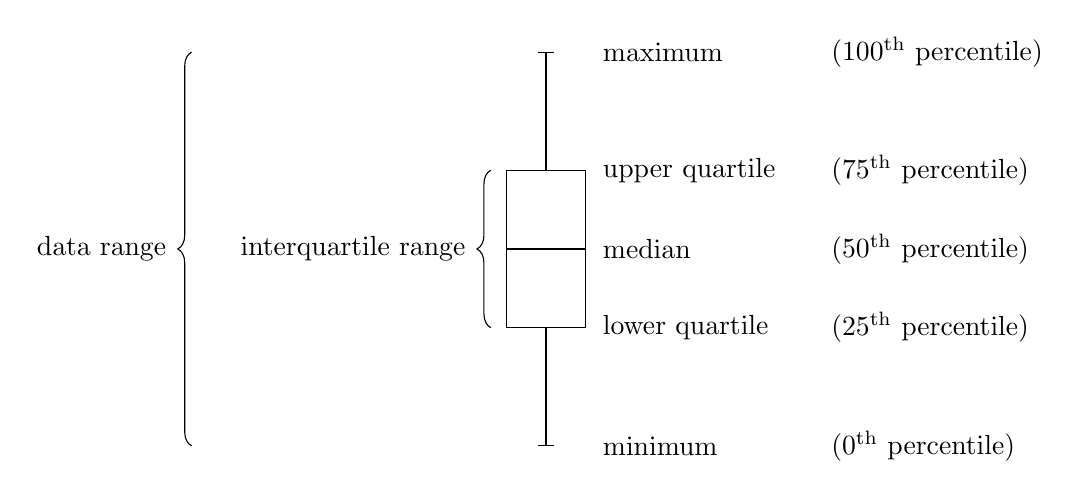
\begin{tikzpicture}
      \draw[thick] (-0.5, 0) -- (0.5, 0);
      \draw (-0.5, -1) rectangle (0.5, 1);
      \draw (0, -1) -- (0, -2.5);
      \draw (-0.1, -2.5) -- (0.1, -2.5);
      \draw (0, 1) -- (0, 2.5);
      \draw (-0.1, 2.5) -- (0.1, 2.5);
      \draw (0.6, 2.5) node[anchor=west] {maximum};
      \draw (0.6, 1) node[anchor=west] {upper quartile};
      \draw (0.6, 0) node[anchor=west] {median};
      \draw (0.6, -1) node[anchor=west] {lower quartile};
      \draw (0.6, -2.5) node[anchor=west] {minimum};
      \draw (3.5, 2.5) node[anchor=west] {($100^{\mathrm{th}}$ percentile)};
      \draw (3.5, 1) node[anchor=west] {($75^{\mathrm{th}}$ percentile)};
      \draw (3.5, 0) node[anchor=west] {($50^{\mathrm{th}}$ percentile)};
      \draw (3.5, -1) node[anchor=west] {($25^{\mathrm{th}}$ percentile)};
      \draw (3.5, -2.5) node[anchor=west] {($0^{\mathrm{th}}$ percentile)};
      \draw[decoration={brace,amplitude=0.5em},decorate] (-0.7,-1) -- (-0.7,1);
      \draw (-0.7,0) node[anchor=east,xshift=-0.2cm] {interquartile range};
      \draw[decoration={brace,amplitude=0.5em},decorate] (-4.5,-2.5) -- (-4.5,2.5);
      \draw (-4.5,0) node[anchor=east,xshift=-0.2cm] {data range};
    \end{tikzpicture}
  \end{center}
%   \begin{caption*}The box-and-whisker plot along with labels showing how
%     the different percentiles and ranges are represented in the plot.\end{caption*}
\end{figure}
\vspace{1cm}

\begin{wex}{Five number summary}
{Draw a box and whisker diagram for the following data set:
    \begin{equation*}
      \{1,25;\ 1,5;\ 2,5;\ 2,5;\ 3,1;\ 3,2;\ 4,1;\ 4,25;\ 4,75;\ 4,8;\ 4,95;\ 5,1\}
    \end{equation*}
}{
  \westep{Determine the minimum and maximum}

  Since the data set is already sorted, we can read off the minimum as
  the first value ($1,25$) and the maximum as the last value ($5,1$).

  \westep{Determine the quartiles}

  There are $12$ values in the data set. Using the percentile formula,
  we can determine that the median lies between the $6^{\mathrm{th}}$ and $7^{\mathrm{th}}$
  values, making it
  \begin{equation*}
    \frac{3,2 + 4,1}{2} = 3,65
  \end{equation*}

  The first quartile lies between the $3^{\mathrm{rd}}$ and $4^{\mathrm{th}}$ values, making
  it
  \begin{equation*}
    \frac{2,5 + 2,5}{2} = 2,5
  \end{equation*}

  The third quartile lies between the $9^{\mathrm{th}}$ and $10^{\mathrm{th}}$ values, making
  it
  \begin{equation*}
    \frac{4,75 + 4,8}{2} = 4,775
  \end{equation*}

  This provides the five number summary of the data set and allows us
  to draw the following box-and-whisker plot.

  \begin{center}
    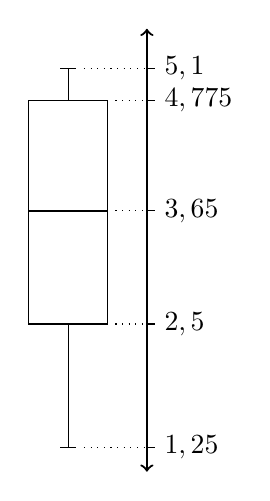
\begin{tikzpicture}[yscale=1.25]
      \def\median{3.65}
      \def\firstquartile{2.5}
      \def\thirdquartile{4.775}
      \def\minimum{1.25}
      \def\maximum{5.1}

      \draw (-0.5, \firstquartile) rectangle (0.5, \thirdquartile);
      \draw[thick] (-0.5, \median) -- (0.5, \median);
      \draw (0,    \firstquartile) -- (0,   \minimum);
      \draw (-0.1, \minimum) -- (0.1,       \minimum);
      \draw (0,    \thirdquartile) -- (0,   \maximum);
      \draw (-0.1, \maximum) -- (0.1,       \maximum);

      \draw[thick,<->] (1,1) -- (1,5.5);

      \foreach \y in {\minimum, \firstquartile, \median, \thirdquartile, \maximum} {
        \draw (1, \y) -- (1.1, \y);
      }
      \foreach \y/\txt in {\minimum/{1,25}, \firstquartile/{2,5}, \median/{3,65}, \thirdquartile/{4,775}, \maximum/{5,1}} {
        \draw (1.1, \y) node[anchor=west] {$\txt$};
      }
      \draw[dotted] (0.2, \maximum) -- (1, \maximum);
      \draw[dotted] (0.6, \thirdquartile) -- (1, \thirdquartile);
      \draw[dotted] (0.6, \median)  -- (1, \median);
      \draw[dotted] (0.6, \firstquartile) -- (1, \firstquartile);
      \draw[dotted] (0.2, \minimum) -- (1, \minimum);
    \end{tikzpicture}
  \end{center}
}
\end{wex}

\begin{exercises}{}{
    \begin{enumerate} [itemsep=6pt, label=\textbf{\arabic*}.]

    \item Lisa is working in a computer store. She sells the following
      number of computers each month:
      \begin{equation*}
        \{27;\ 39;\ 3;\ 15;\ 43;\ 27;\ 19;\ 54;\ 65;\ 23;\ 45;\ 16\}
      \end{equation*}
      Give the five number summary and box-and-whisker plot of Lisa's
      sales.

    \item Zithulele works as a telesales person. He keeps a record of the
      number of sales he makes each month. The data below show how much he
      sells each month.
      \begin{equation*}
        \{49;\ 12;\ 22;\ 35;\ 2;\ 45;\ 60;\ 48;\ 19;\ 1;\ 43;\ 12\}
      \end{equation*}
      Give the five number summary and box-and-whisker plot of Zithulele's
      sales.

    \item Hannah has worked as a florist for nine months. She sold the
      following number of wedding bouquets:
      \begin{equation*}
        \{16;\ 14;\ 8;\ 12;\ 6;\ 5;\ 3;\ 5;\ 7\}
      \end{equation*}
      Give the five number summary of Hannah's sales.
    \item Use the diagram below to determine the five number summary:
      \begin{enumerate}[noitemsep, label=\textbf{(\alph*)} ]
      \item \raisebox{-2cm}{
          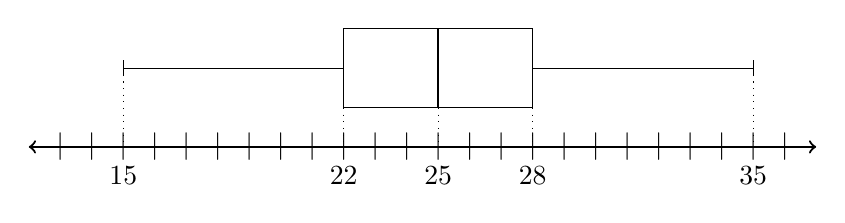
\begin{tikzpicture}[xscale=0.4]
            \def\median{25}
            \def\firstquartile{22}
            \def\thirdquartile{28}
            \def\minimum{15}
            \def\maximum{35}

            \draw (\firstquartile, -0.5 ) rectangle ( \thirdquartile,0.5);
            \draw[thick] ( \median,-0.5) -- ( \median,0.5);
            \draw (    \firstquartile, 0) -- (\minimum,0   );
            \draw ( \minimum, -0.1) -- (       \minimum, 0.1);
            \draw (  \thirdquartile, 0) -- (   \maximum, 0);
            \draw ( \maximum, -0.1) -- (      \maximum, 0.1 );

            \draw[thick,<->] (12,-1) -- (37,-1);

            \foreach \x in {\minimum, \firstquartile, \median, \thirdquartile, \maximum} {
              \draw (\x,-1.6) -- (\x, -1.6) node[anchor=south] {$\x$};
            }

            \foreach \x in {13,14,...,36} {
              \draw (\x,-1.3) -- (\x, -1.3) node[anchor=south] {$|$};
            }
            \draw[dotted] ( \maximum, 0) -- ( \maximum, -1);
            \draw[dotted] ( \thirdquartile, 0) -- ( \thirdquartile, -1);
            \draw[dotted] (\median, 0)  -- ( \median, -1);
            \draw[dotted] (\firstquartile, 0) -- ( \firstquartile, -1);
            \draw[dotted] ( \minimum, 0) -- ( \minimum, -1);
          \end{tikzpicture}
        }
      \item \raisebox{-2cm}{
          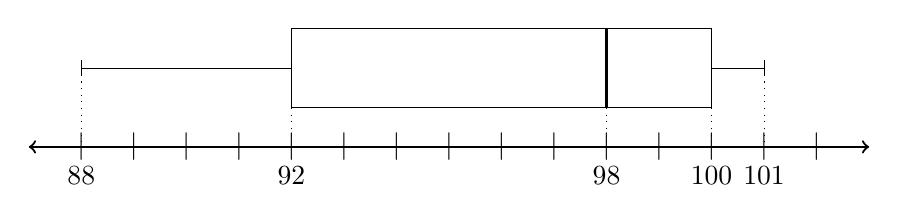
\begin{tikzpicture}[xscale=0.667]
            \def\median{98}
            \def\firstquartile{92}
            \def\thirdquartile{100}
            \def\minimum{88}
            \def\maximum{101}

            \draw (\firstquartile, -0.5 ) rectangle ( \thirdquartile,0.5);
            \draw[thick] ( \median,-0.5) -- ( \median,0.5);
            \draw (    \firstquartile, 0) -- (\minimum,0   );
            \draw ( \minimum, -0.1) -- (       \minimum, 0.1);
            \draw (  \thirdquartile, 0) -- (   \maximum, 0);
            \draw ( \maximum, -0.1) -- (      \maximum, 0.1 );

            \draw[thick,<->] (87,-1) -- (103,-1);

            \foreach \x in {\minimum, \firstquartile, \median, \thirdquartile, \maximum} {
              \draw (\x,-1.6) -- (\x, -1.6) node[anchor=south] {$\x$};
            }

            \foreach \x in {88,89,...,102} {
              \draw (\x,-1.3) -- (\x, -1.3) node[anchor=south] {$|$};
            }
            \draw[dotted] ( \maximum, 0) -- ( \maximum, -1);
            \draw[dotted] ( \thirdquartile, 0) -- ( \thirdquartile, -1);
            \draw[dotted] (\median, 0)  -- ( \median, -1);
            \draw[dotted] (\firstquartile, 0) -- ( \firstquartile, -1);
            \draw[dotted] ( \minimum, 0) -- ( \minimum, -1);
          \end{tikzpicture}
        }
      \end{enumerate}
    \end{enumerate}
\practiceinfo
\par 
\par \begin{tabular}[h]{cccccc}
(1.) 00k4&  (2.) 00k5&  (3.) 00k6&  (4.) 00k7\end{tabular}
}
\end{exercises}


\summary{VMdvy}

\begin{itemize}[itemsep=6pt]
\item Data refer to the pieces of information that have been observed and recorded, from an experiment or a survey. 

\item Quantitative data are data that can be written as numbers.  Quantitative data can be discrete or continuous.

\item Qualitative data are data that cannot be written as numbers.  There are two common types of qualitative data: categorical and anecdotal data. 

\item The mean is the sum of a set of values divided by the number of values in the set. 
  \begin{align*}
    \overline{x} &= \frac{1}{n}\sum_{i=1}^n x_i \\
                 &= \frac{x_1 + x_2 + \cdots + x_n}{n}
  \end{align*}

\item The median of a data set is the value in the central position, when the data set has 
been arranged from the lowest to the highest value.  If there are an odd number of data, the median will be equal to one of the values in the data set. If there are an even number of data, the median will lie half way between two values in the data set. 

\item The mode of a data set is the value that occurs most often in the set. 

\item An outlier is a value in the data set that is not typical of the rest of the set. It is 
usually a value that is much greater or much less than all the other values in the data set.

\item Dispersion is a general term for different statistics that describe how values are distributed around the centre. 

\item The range of a data set is the difference between the maximum and minimum values 
in the set. 

\item The $p^{\mathrm{th}}$ percentile is the value, $v$, that divides a data set into two parts, such that 
$p\%$ of the values in the data set are less than $v$ and $100 − p\%$ of the 
values are greater than $v$. 

The general formula for finding the $p^{\mathrm{th}}$ percentile in an ordered data set with $n$ values is 
\begin{equation*}
  r = \frac{p}{100}\left(n-1\right)+1
\end{equation*}

\item The quartiles are the three data values that divide an ordered data set into four groups, where each group contains an equal number of data values. The lower quartile is denoted $Q1$, the median is $Q2$ and the upper quartile is $Q3$.

\item The interquartile range is a measure of dispersion, which is calculated by subtracting the lower (first) quartile from the upper (third) quartile. This gives the range of the middle half of the data set.

\item The semi interquartile range is half of the interquartile range. 

\item The five number summary consists of the minimum value, the maximum value and the three quartiles ($Q1$, $Q2$ and $Q3$). 

\item The box-and-whisker plot is a graphical representation of the five number summary.
\end{itemize}

\begin{eocexercises}{}
  \begin{enumerate}[itemsep=6pt, label=\textbf{\arabic*}.]

  \item 
  In a park, the tallest $7$ trees in a park have heights in metres of
    $41$; $60$; $47$; $42$; $44$; $42$; and $47$. Find the median of
    their heights.

  \item The students in Ndeme's class have the following ages: $5$;
    $6$; $7$; $5$; $4$; $6$; $6$; $6$; $7$; $4$. Find the mode of
    their ages.

  \item An engineering company has designed two different types of
    engines for motorbikes. The two different motorbikes are tested
    for the time (in seconds) it takes for them to accelerate from $0$
    km/h to $60$ km/h.

    \begin{center}
      \begin{tabular}{|@{\hspace{0.1cm}}c@{\hspace{0.1cm}}|@{\hspace{0.1cm}}c@{\hspace{0.1cm}}|@{\hspace{0.1cm}}c@{\hspace{0.1cm}}|@{\hspace{0.1cm}}c@{\hspace{0.1cm}}|@{\hspace{0.1cm}}c@{\hspace{0.1cm}}|@{\hspace{0.1cm}}c@{\hspace{0.1cm}}|@{\hspace{0.1cm}}c@{\hspace{0.1cm}}|@{\hspace{0.1cm}}c@{\hspace{0.1cm}}|@{\hspace{0.1cm}}c@{\hspace{0.1cm}}|@{\hspace{0.1cm}}c@{\hspace{0.1cm}}|@{\hspace{0.1cm}}c@{\hspace{0.1cm}}|} \hline
     
        & \textbf{Test 1} & \textbf{Test 2} & \textbf{Test 3} & \textbf{Test 4} & \textbf{Test 5} & \textbf{Test 6} & \textbf{Test 7} &\textbf{Test 8} & \textbf{Test 9} & \textbf{Test 10} \\\hline
        \textbf{Bike 1} & $1,55$ & $1,00$ & $0,92$ & $0,80$ & $1,49$ & $0,71$ & $1,06$ & $0,68$ & $0,87$ & $1,09$ \\\hline
        \textbf{Bike 2} & $0,9$ & $1,0$ & $1,1$ & $1,0$ & $1,0$ & $0,9$ & $0,9$ & $1,0$ & $0,9$ & $1,1$ \\\hline

      \end{tabular}
    \end{center}
\vspace {8pt}\\
\begin{enumerate}[noitemsep, label=\textbf{(\alph*)} ]
    \item Which measure of central tendency should be used for this
      information?
    \item Calculate the measure of central tendency that you chose in
      the previous question, for each motorbike.
    \item Which motorbike would you choose based on this information?
      Take note of the accuracy of the numbers from each set of tests.
    \end{enumerate}

  \item In a traffic survey, a random sample of $50$ motorists were
    asked the distance they drove to work daily. This information is
    shown in the table below.\\
    \begin{center}
      \begin{tabular}{|c|c|} \hline
     
        \textbf{Distance (km)} & \textbf{Count} \\ \hline

        $0 < d \leq 5$ & $4$ \\ \hline
        $5 < d \leq 10$ & $5$ \\\hline
        $10 < d \leq 15$ & $9$ \\\hline
        $15 < d \leq 20$ & $10$ \\\hline
        $20 < d \leq 25$ & $7$ \\\hline
        $25 < d \leq 30$ & $8$ \\\hline
        $30 < d \leq 35$ & $3$ \\\hline
        $35 < d \leq 40$ & $2$ \\\hline
        $40 < d \leq 45$ & $2$ \\\hline

      \end{tabular}
    \end{center}
\vspace {8pt}\\
     \begin{enumerate}[noitemsep, label=\textbf{(\alph*)} ]
    \item Find the approximate mean of the data.
    \item What percentage of samples had a speed of
      \begin{enumerate}[noitemsep, label=\textbf{\roman*}. ]
      \item less than $15$ km?
      \item more than $30$ km?
      \item between $16$ km and $30$ km daily?
      \end{enumerate}
\item Draw a histogram to represent the data
    \end{enumerate}

  \item A company wanted to evaluate the training programme in its
    factory. They gave the same task to trained and untrained
    employees and timed each one in seconds.
\\
    \begin{center}
      \begin{tabular}{|l|c|c|c|c|c|} \hline

        \textbf{Trained} & 121 & 137 & 131 & 135 & 130 \\ \hline
                         & 128 & 130 & 126 & 132 & 127 \\\hline
                         & 129 & 120 & 118 & 125 & 134 \\\hline

        \textbf{Untrained} & 135 & 142 & 126 & 148 & 145 \\\hline
                           & 156 & 152 & 153 & 149 & 145 \\\hline
                           & 144 & 134 & 139 & 140 & 142 \\\hline

      \end{tabular}
    \end{center}
\vspace {8pt}\\
    \begin{enumerate}[noitemsep, label=\textbf{(\alph*)} ]
    \item Find the medians and quartiles for both sets of data.
    \item Find the interquartile range for both sets of data.
    \item Comment on the results.
    \item Draw a box-and-whisker diagram for each data set to illustrate the five number summary.
    \end{enumerate}

  \item A small firm employs nine people. The annual salaries of the employers are:
\\
    \begin{center}
      \begin{tabular}{|r|r|r|} \hline
        R~$600~000$ & R~$250~000$ & R~$200~000$ \\\hline
        R~$120~000$ & R~$100~000$ & R~$100~000$ \\\hline
        R~$100~000$ &  R~$90~000$ &  R~$80~000$ \\\hline
      \end{tabular}
    \end{center}
\vspace {8pt}\\
    \begin{enumerate}[noitemsep, label=\textbf{(\alph*)} ]
    \item Find the mean of these salaries.
    \item Find the mode.
    \item Find the median.
    \item Of these three figures, which would you use for
      negotiating salary increases if you were a trade union
      official? Why?
    \end{enumerate}

  \end{enumerate}
\practiceinfo
\par 
\par \begin{tabular}[h]{cccccc}
(1.) 00k8&  (2.) 00k9&  (3.) 00ka&  (4.) 00kb&  (5.) 00kc&  (6.) 00kd\end{tabular}
\end{eocexercises}
